\documentclass[conference]{IEEEtran}
\IEEEoverridecommandlockouts
\usepackage{cite}
\usepackage{amsmath,amssymb,amsfonts}
\usepackage{graphicx}
\usepackage{textcomp}
\usepackage{xcolor}
\usepackage{booktabs}
\usepackage{url}

\def\BibTeX{{\rm B\kern-.05em{\sc i\kern-.025em b}\kern-.08em
    T\kern-.1667em\lower.7ex\hbox{E}\kern-.125emX}}

\begin{document}

\title{Detecting Recyclable Waste on a Conveyor Belt with YOLOv8: A Comparison of Data Augmentation Policies}

\author{
\IEEEauthorblockN{Julia Maldonado, Alejandro Valle, Mar\'ia Gabriela Di Grazia, Byron Garc\'ia}
\IEEEauthorblockA{
Specialization Program in Artificial Intelligence (CEIA)\\
Faculty of Engineering, University of Buenos Aires (FIUBA)\\
Computer Vision II --- Group 6
}
}

\maketitle

\begin{abstract}
Collection centers receive mixed waste whose manual sorting is slow and costly.
This work proposes a computer vision system that, installed over a conveyor belt, detects and
classifies waste into six categories (biodegradable, cardboard, glass, metal, paper and
plastic) in order to prioritize the extraction of the materials with the highest recycling
value. We trained and compared four configurations -- two YOLOv8 variants (n and s) under two
data augmentation policies -- on a dataset of 10,464 images (Garbage Classification 3,
Roboflow). The proposed augmentation policy, designed from a quantitative analysis of the
dataset's shortcomings (orientation, lighting and sharpness), improved mAP@0.5:0.95 by
1.2 points (YOLOv8s) and 0.7 points (YOLOv8n) over the default Ultralytics configuration, with
YOLOv8s + proposed reaching 0.650 mAP@0.5 and 55 FPS on a T4 GPU.
\end{abstract}

\begin{IEEEkeywords}
object detection, YOLOv8, waste classification, data augmentation, computer vision, recycling.
\end{IEEEkeywords}

\section{Introduction}

Busy cities generate large amounts of mixed waste. Sorting it manually, material by material,
is slow and costly, and much of the recyclable material loses commercial value because it is
not identified and extracted in time during processing. Classifying directly on the street
during collection is impractical because of lighting and motion conditions; it is more viable
to automate classification once the waste reaches a collection center or processing plant,
where it can pass along a conveyor belt under controlled camera conditions.

The goal of this work is to design and evaluate a deep-learning-based object detection system
that, over a conveyor belt, identifies the category of each item in real time and allows the
extraction of the highest-value materials (for example aluminum, PET or cardboard) to be
prioritized, instead of requiring exhaustive separation of 100\% of the flow. The scope of
this work is the computer vision problem --- detecting and classifying the different types of
waste --- leaving the physical implementation of the separation mechanism (a robotic arm or
compressed air) as a future extension.

As a real-world precedent, Koskinopoulou et al.~\cite{koskinopoulou2021} describe a computer
vision categorization system for the industrial robotic separation of recyclable waste,
deployed and evaluated in a real waste processing plant under demanding industrial conditions,
using a low-cost deep-learning-based vision module. In industry, Recycleye reports a
deployment at the re3 materials recovery facility (MRF) in Reading, United Kingdom, with 99\%
purity of the separated material versus 96\% on the human reference sorting line and up to 55
picks per minute~\cite{recycleye2022}. Both precedents support the viability of a computer
vision approach to this task, although the industry figures are not independently audited,
unlike the metrics reported in this work.

\section{Methodology}

\subsection{Dataset and Processing}

We used the public Garbage Classification 3 dataset (v2, YOLOv8 format) from
Roboflow~\cite{roboflow2024}, with 10,464 images annotated in six classes: biodegradable,
cardboard, glass, metal, paper and plastic. Before training, the raw export was audited to
discard corrupt images and to fix or remove defective annotations --- a necessary step because
Roboflow exports can contain labeling errors that silently harm training. The dataset was
re-split into our own 70/20/10 (train/val/test) partition instead of keeping Roboflow's, which
was class-imbalanced and would have invalidated the per-class evaluation. The test set was
kept held out and unaugmented until the final evaluation.

\subsection{Augmentation Policy}

The augmentation techniques were chosen from a quantitative analysis of the processed dataset
--- not from generic assumptions --- measuring brightness, sharpness, color and class balance.
The analysis showed that the dataset lacks dark or blurry images, conditions expected in real
conveyor belt video, and that the observed class imbalance is due to the number of objects per
photo rather than the number of photos per class. From these findings we defined two
configurations (\emph{arms}) to compare: \texttt{ultralytics\_defaults}, the default
Ultralytics augmentation~\cite{ultralytics2023} (mosaic, HSV jitter, horizontal flip,
translation and scale), and \texttt{proposed}, which adds vertical flip, darkening (brightness
reduction of up to 40\% with probability 0.3), motion blur and Gaussian blur, to cover the
measured gaps in orientation, lighting and sharpness, implemented with
Albumentations~\cite{buslaev2020}. Augmentation is applied \emph{online} during training from
a single shared configuration file, so all runs use exactly the same policy and the test set
is never augmented by accident.

\subsection{Training and Evaluation}

We fine-tuned two pre-trained YOLOv8 variants~\cite{ultralytics2023} --- YOLOv8n and YOLOv8s
--- under each of the two augmentation policies, yielding four trained configurations. Each
model was trained for 50 epochs with batch size 16 and a fixed seed (42) on a T4 GPU (Google
Colab). Evaluation was performed on the held-out test set, reporting mAP@0.5, mAP@0.5:0.95, F1
and end-to-end inference latency (200 test images, processed one at a time), measured on both
a T4 GPU and a laptop CPU (Intel i5-1135G7).

\section{Experimental Results and Analysis}

Table~\ref{tab:metrics} summarizes the metrics of the four configurations on the test set.
The \texttt{proposed} policy outperformed \texttt{ultralytics\_defaults} on both
architectures: +1.2 points of mAP@0.5:0.95 for YOLOv8s and +0.7 points for YOLOv8n. The
improvement was observed in five of the six classes on both models, with a single minor
exception in CARDBOARD (-0.008), suggesting that the darkening and blur added by the proposed
policy help consistently without introducing a relevant regression.

\begin{table}[htbp]
\caption{Metrics by model and recipe (test set)}
\begin{center}
\begin{tabular}{llccc}
\toprule
\textbf{Model} & \textbf{Recipe} & \textbf{mAP@0.5} & \textbf{mAP@.5:.95} & \textbf{F1} \\
\midrule
YOLOv8s & proposed             & 0.650 & 0.467 & 0.650 \\
YOLOv8s & ultralytics\_defaults & 0.645 & 0.455 & 0.646 \\
YOLOv8n & proposed             & 0.629 & 0.443 & 0.625 \\
YOLOv8n & ultralytics\_defaults & 0.622 & 0.435 & 0.617 \\
\bottomrule
\end{tabular}
\label{tab:metrics}
\end{center}
\end{table}

YOLOv8s outperformed YOLOv8n in all six classes under both recipes, at the cost of higher
latency: on the T4 GPU, YOLOv8s + proposed processed each image in 18.1~ms (55~FPS) versus
10.2~ms (98~FPS) for YOLOv8n + proposed. On CPU (Intel i5-1135G7, \texttt{proposed} weights),
YOLOv8n reached 68.9~ms (14.5~FPS) versus 177.3~ms (5.6~FPS) for YOLOv8s --- a 2.6$\times$
difference that matters for deployment without a dedicated GPU.

The recommended model is YOLOv8s with the \texttt{proposed} policy, as it has the best
mAP@0.5:0.95 and F1 of the set and runs in real time on GPU (55~FPS). For deployment without
a GPU we recommend YOLOv8n + \texttt{proposed} as an alternative, with a 2.4-point drop in
mAP@0.5:0.95 in exchange for being 2.6$\times$ faster on CPU. The worst-performing classes on
both models are BIODEGRADABLE, CARDBOARD and PAPER (mAP@0.5:0.95 between 0.36 and 0.43 for
YOLOv8s), consistent with the visual variability of those materials.

\subsection{Demonstration on a Simulated Belt}

To illustrate how the system works without a physical belt, we built a simulation: 11 images
from the test set (randomly chosen with a fixed seed), each resized to a 420~px square, slide
from left to right over a 1280$\times$540~px belt background at 30~FPS for 20~s (600 frames),
as if passing in front of a fixed camera. The recommended model (YOLOv8s + \texttt{proposed},
confidence threshold 0.25) runs frame by frame, as an online system would.
Fig.~\ref{fig:demo} shows six representative frames.

\begin{figure*}[t]
\centering
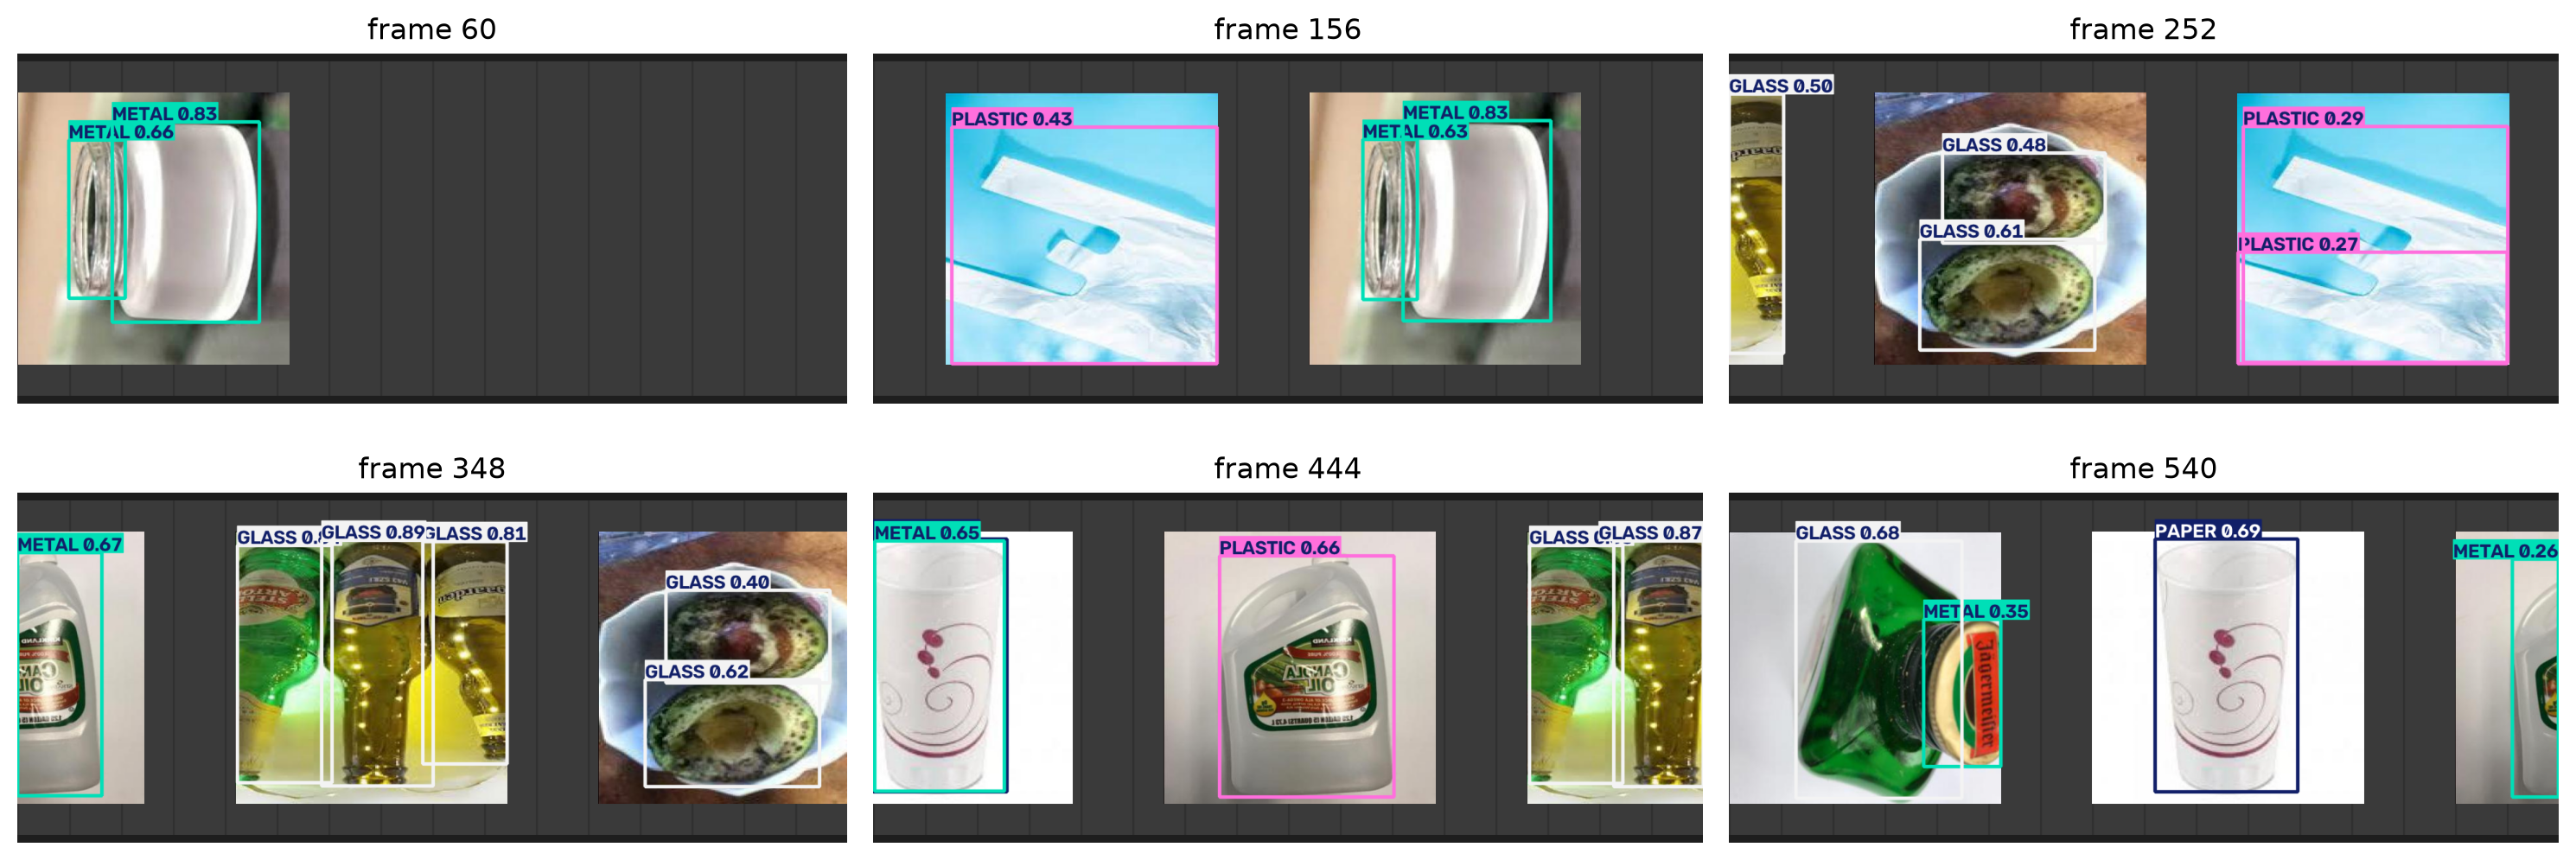
\includegraphics[width=\textwidth]{demo_frames.png}
\caption{Six frames of the simulated belt demonstration, with the detections of the
YOLOv8s + \texttt{proposed} model. Correct detections (glass bottles, paper cup) and class
confusions, particularly METAL, can be seen.}
\label{fig:demo}
\end{figure*}

Per-frame latency (preprocessing, inference and NMS) was 22.9~ms on average (43.7~FPS) and
13.3~ms at the 95th percentile, running on the integrated GPU (MPS backend) of a MacBook Pro.
That the mean exceeds the 95th percentile indicates that a few initial frames were much
slower (device warm-up); in steady state the model stayed above the 30~FPS of the simulated
video.

\begin{table}[htbp]
\caption{Detections per class in the demonstration (per-frame count)}
\begin{center}
\begin{tabular}{lcc}
\toprule
\textbf{Class} & \textbf{Detections} & \textbf{Mean confidence} \\
\midrule
GLASS         & 1241 & 0.616 \\
METAL         &  746 & 0.617 \\
PLASTIC       &  482 & 0.487 \\
PAPER         &  188 & 0.686 \\
BIODEGRADABLE &   53 & 0.554 \\
CARDBOARD     &    5 & 0.396 \\
\bottomrule
\end{tabular}
\label{tab:demo}
\end{center}
\end{table}

Table~\ref{tab:demo} counts detections \emph{per frame}: the same object appears in many
consecutive frames, so the table reflects the images that traveled along the belt and not the
number of distinct objects (which would require tracking; see Conclusions). In the inspected
frames we observed two behaviors. On one hand, objects with a clear appearance are classified
with high confidence, for example the green glass bottles (0.81 to 0.89). On the other hand,
there are confusions that the aggregate test metrics do not reveal: the same white plastic
jug was labeled PLASTIC (0.66) in one frame and METAL (0.67) in another; a paper cup was
labeled PAPER (0.69) and, when entering from the edge of the belt partially cropped, METAL
(0.65); a glass jar was labeled METAL; and avocado scraps in a bowl were labeled GLASS instead
of BIODEGRADABLE. The class becomes unstable when the object appears cut off at the edge of
the frame, a scenario that testing on complete images does not measure. CARDBOARD was almost
never detected (5 detections, mean confidence 0.396), consistent with its low test
performance. These observations are qualitative and based on 11 distinct images, so they do
not replace the quantitative evaluation of Table~\ref{tab:metrics}.

Limitations: each model and recipe was trained only once, so the reported differences were
not subjected to a statistical significance test. Of the four recipes defined in the
augmentation policy, only two (\texttt{ultralytics\_defaults} and \texttt{proposed}) were
actually trained; \texttt{no\_augmentation} and \texttt{proposed\_low\_saturation} remain as
future work. Confusion matrices were computed on the validation set, not the test set.
Moreover, the dataset used, although realistic, does not fully replicate the level of visual
clutter (overlapping objects, partial occlusions) that the specialized literature documents in
real conveyor belt video~\cite{bashkirova2022}; validating the recommended model against our
own belt images, closer to that scenario, is a natural step before a production deployment.

\section{Conclusions}

\begin{enumerate}
\item An augmentation policy designed from quantitatively measured dataset gaps (orientation,
lighting, sharpness) consistently improves mAP@0.5:0.95 over the Ultralytics defaults, on both
architectures evaluated, without collecting more data.

\item YOLOv8s offers better accuracy than YOLOv8n in all six classes under both recipes, but
at a relevant latency cost on CPU (2.6$\times$ slower than YOLOv8n), so the choice between
them depends directly on the hardware available at the collection center.

\item Re-splitting the dataset instead of using Roboflow's original partition was necessary to
obtain a reliable per-class evaluation, given the imbalance detected in the original
partition.

\item The BIODEGRADABLE, CARDBOARD and PAPER classes concentrate the lowest performance of the
system, suggesting that visual ambiguity between organic and fiber materials is the main
bottleneck to address in a future iteration, more than the detector architecture itself.

\item The simulated belt demonstration ran at 43.7~FPS on an integrated GPU (MPS), above the
30~FPS of the video, but showed confusions that the test set does not reveal, mainly METAL
versus PLASTIC, PAPER and GLASS, and unstable classes when the object is cut off at the edge
of the frame. This reinforces that the next step is validating with our own belt images and
with partially visible objects.

\item As future work, the architecture can be extended with object tracking to avoid counting
the same item twice in video, and by directly evaluating the physical implementation of the
separation mechanism, which was outside the scope of this work.
\end{enumerate}

\bibliographystyle{ieeetr}
\bibliography{references}

\end{document}
